\chapter{トレースログ可視化ツール TraceLogVisualizer の設計}

\section{開発方針}
TLVの開発目標は,汎用性と拡張性を備えることである.

ここで,汎用性とは,可視化表示したいトレースログの形式を制限しないことであり,可視化表示メカニズムをトレースログの形式に依存させないことによって実現する.
具体的には,まず,トレースログを抽象的に扱えるように,トレースログを一般化した標準形式トレースログを定義する.
そして,任意の形式のトレースログを標準形式トレースログに変換する仕組みを,変換ルールとして形式化して定義出来る用にする.
これにより,変換ルールの記述で任意のトレースログが標準形式トレースログに変換することができるため,あらゆるトレースログの可視化に対応することが可能となる.

次に,拡張性とは,トレースログに対応する可視化表現をユーザレベルで拡張出来ることを表し,トレースログから可視化表示を行う仕組みを抽象化し,それを可視化ルールとして形式化して定義出来るようにすることで実現する.
可視化ルールを記述することにより,トレースログ内の任意の情報を自由な表現方法で可視化することが可能になる.


\section{標準形式トレースログ}

本節では,標準形式トレースログを定義するために行ったトレースログの抽象化と,標準形式トレースログの定義について述べる.

\subsection{トレースログの抽象化}

標準形式トレースログを提案するにあたり,トレースログの抽象化を行った.

はじめに,トレースログを時系列にイベントを記録したものと考えた.
次に,イベントとはイベント発生源の属性の変化,イベント発生源の振る舞いと考えた.
ここで,イベント発生源をリソースと呼称し,固有の識別子をもつものとする.
つまりリソースとは,イベントの発生源であり,名前を持ち,固有の属性をもつものと考えることが出来る.
リソースは型により属性,振る舞いを特徴付けられる.
ここでリソースの型をリソースタイプと呼称する.
属性とはリソースが固有にもつ文字列,数値,真偽値で表されるスカラーデータとし,振る舞いとはリソースの行為であるとする.
振る舞いは任意の数のスカラーデータを引数として受け取ることができる.
リソースタイプとリソースの関係は,オブジェクト指向におけるクラスとオブジェクトの関係に類似しており,属性と振る舞いはメンバ変数とメソッドに類似している.
ただし,振る舞いはリソースのなんらかの行為を表現しており,メソッドの,メンバ変数を操作するための関数や手続きを表す概念とは異なる.
主に振る舞いは,属性の変化を伴わないイベントを表現するために用いる.
振る舞いの引数は,図形描画の際の条件,あるいは描画材料として用いられることを想定している.

図\ref{fig:resourceTypeSample}と図\ref{fig:resourceSample}に,リソースタイプとリソースを図で表現した例を示す.
さらに,図\ref{fig:resourceTypeSampleByTask}に,RTOS(Real-time operating system)におけるタスクの概念をリソースタイプとして表現した例を,図\ref{fig:resourceSampleByTask}にリソースタイプTaskのリソースの例としてMainTaskを示す.

トレースログの抽象化を以下にまとめる.

\begin{description}
\item[トレースログ] \mbox{} \\
時系列にイベントを記録したもの.
\item[イベント] \mbox{} \\
リソースの属性の値の変化,リソースの振る舞い.
\item[リソース] \mbox{} \\
イベントの発生源.固有の名前,属性をもつ.
\item[リソースタイプ] \mbox{} \\
リソースの型.リソースの属性,振る舞いを特徴付ける.
\item[属性] \mbox{} \\
リソースが固有にもつ情報.文字列,数値,真偽値のいずれかで表現されるスカラーデータで表される.
\item[振る舞い] \mbox{} \\
リソースの行為.主に属性の値の変化を伴わない行為をイベントとして記録するために用いることを想定している.
\end{description}

\begin{figure}[h]
\begin{tabular}{cc}
\begin{minipage}{0.5\hsize}
\begin{center}
\includegraphics[scale=0.5]{img/resourceTypeSample.eps}
\caption{リソースタイプ}
\label{fig:resourceTypeSample}
\end{center}
\end{minipage}
\begin{minipage}{0.5\hsize}
\begin{center}
\includegraphics[scale=0.5]{img/resourceSample.eps}
\caption{リソース}
\label{fig:resourceSample}
\end{center}
\end{minipage}
\end{tabular}
\end{figure}

\begin{figure}[h]
\begin{tabular}{ccc}
\begin{minipage}{0.35\hsize}
\begin{center}
\includegraphics[scale=0.5]{img/resourceTypeSampleByTask.eps}
\caption{タスクをリソースタイプTaskとして表現した例}
\label{fig:resourceTypeSampleByTask}
\end{center}
\end{minipage}
\begin{minipage}{0.25\hsize}
\mbox{}\\
\end{minipage}
\begin{minipage}{0.3\hsize}
\begin{center}
\includegraphics[scale=0.5]{img/resourceSampleByTask.eps}
\caption{リソースタイプTaskのリソースMainTaskの例}
\label{fig:resourceSampleByTask}
\end{center}
\end{minipage}
\end{tabular}
\end{figure}

\clearpage

\subsection{標準形式トレースログの定義}

本小節では,前小節で抽象化したトレースログを標準形式トレースログとして形式化する.
標準形式トレースログの定義にはEBNF(Extended Backus Naur Form)および終端記号として正規表現を用いる.
正規表現はスラッシュ記号(/)で挟むものとする.

前小節によればトレースログとは時系列にイベントを記録したものであるので,1つのログには時刻とイベントが含まれるべきである.
トレースログが記録されたファイルのデータを\verb|TraceLog|,\verb|TraceLog|を改行記号で区切った1行を\verb|TraceLogLine|とする.

\begin{EBNF}
TraceLog = { TraceLogLine };
TraceLogLine = "[",Time,"]",Event,"\n";
\end{EBNF}

\verb|TraceLogLine|は"\verb|[|","\verb|]|"で時刻を囲み,その後ろにイベントを記述するものとする.

時刻は\verb|Time|として定義され,数値とアルファベットで構成される.

\begin{EBNF}
Time = /[0-9a-Z]+/;
\end{EBNF}

アルファベットが含まれるのは,10進数以外の時刻を表現できるようにするためである.
これは,時刻の単位として「秒」以外のもの,たとえば「実行命令数」などを表現出来るように考慮したためである.
この定義から時刻には2進数から36進数までを指定できることがわかる.

前小節にてイベントを「リソースの属性の値の変化,リソースの振る舞い」と抽象化した.
そのため,\verb|Event|を次のように定義した.

\begin{EBNF}
Event = Resource,".",(AttributeChange|BehaviorHappen);
\end{EBNF}

リソースはリソース名による直接指定、あるいは型名と属性条件による条件指定の2通りの指定方法を用意した.

\begin{EBNF}
Resource = ResourceName
         | ResourceTypeName,"(",AttributeCondition,")";
ResourceName = Name;
ResourceTypeName = Name;
Name = /[0-9a-Z_]+/;
\end{EBNF}

条件指定の際の\verb|AttributeCondition|は次のように定義する.

\begin{EBNF}
AttributeCondition = BooleanExpression;
BooleanExpression = Boolean
   |ComparisonExpression
   |BooleanExpression,[{LogicalOpe,BooleanExpression}]
   |"(",BooleanExpression,")";
ComparisonExpression = AttributeName,ComparisonOpe,Value;
Boolean = "true"|"false";
LogicalOpe = "&&"|"||";
ComparisonOpe = "=="|"!="|"<"|">"|"<="|">=";
\end{EBNF}

{\tt AttributeName}はリソースの名前である.

\begin{EBNF}
AttributeName = Name;
\end{EBNF}

{\tt Event}の定義にて,\verb|AttributeChange|は属性の値の変化を,\verb|BehaviorHappen|は振る舞いを表現している.
これらは,リソースとドット"\verb|.|"でつなげることでそのリソース固有のものであることを示す.
リソースの属性の値の変化と振る舞いは次のように定義した.

\begin{EBNF}
AttributeChange = AttributeName,"=",Value;
Value = /[^"\\]+/;
BehaviorHappen =  BehaviorName,"(",Arguments,")";
BehaviorName = Name;
Arguments = [{Argument,[","]}];
Argument = /[^"\\]*/;
\end{EBNF}

\subsection{標準形式トレースログの例}

前小節の定義を元に記述した標準形式トレースログの例を次に示す.

\begin{File}{標準形式トレースログの例}{standartFormatTraceLogSample}
[2403010]MAIN_TASK.leaveSVC(ena_tex,ercd=0)
[4496099]MAIN_TASK.state=RUNNABLE
[4496802]TASK(state==RUNNING).preempt()
[4496802]TASK(state==RUNNING).state=RUNNABLE
[4496802]TASK(id==2).dispatch()
\end{File}

1行目,3行目,5行目がリソースの振る舞いイベントであり,2行目,4行目が属性の値の変化イベントである.
1行目の振る舞いイベントには引数が指定されており,残りの振る舞いイベントには指定されていない.

1行目,2行目はリソースを名前で直接指定しているが,残りはリソースタイプと属性の条件によってリソースを特定している.

\section{可視化表示メカニズムの抽象化}

前節では,トレースログを一般化し,標準形式トレースログとして定義した.
TLVの可視化表示メカニズムは,この標準形式トレースログにのみ依存するように設計されなければならない.
本節では,可視化表現と可視化表現とトレースログの対応を抽象化する.

\subsection{可視化表現}
\label{subsec:visualization}

TLVにおいて,トレースログの可視化表現とは,x軸を時系列とした2次元直交座標系における図形の描画であるとした.
本小節では,座標系と図形について詳述する.

\subsubsection{座標系}

図形を定義する座標系と表示する座標系は分離する.
これにより,図形を表示環境から独立して定義することが可能になる.
図形を定義する座標系をローカル座標系,表示する座標系をデバイス座標系と呼称する.

また,TLVでは,高さと時間を次元に持つ,ワールド座標系という座標系を導入した.
ローカル座標系で定義された図形は,はじめに,ワールド座標系における,図形を表示すべき時間の領域にマッピングされ,これを表示環境に依存するデバイス座標系にマッピングすることで表示する.
これにより,図形の表示領域を,抽象度の高い時刻で指定することが可能になる.
ここで,ローカル座標系からワールド座標系へのマッピングをワールド変換と呼称する.
また,表示する時間の領域を表示期間と呼称する.
表示期間は開始時刻と終了時刻で表される時刻のペアである.

ローカル座標系において図形の大きさと位置を定義する際は,pixel単位による絶対指定か,ワールド座標系へのマッピング領域に対する割合を\%で指定する相対指定かのいずれかを用いる.

図\ref{fig:coordinate}に座標系の例を,図\ref{fig:shapes}にワールド変換の例を示す.

\begin{figure}[p]
\begin{center}
\includegraphics[scale=0.75]{img/coordinate.eps}
\caption{座標系}
\label{fig:coordinate}
\end{center}
\end{figure}

\begin{figure}[p]
\begin{center}
\includegraphics[scale=0.75]{img/worldTransform.eps}
\caption{ワールド変換}
\label{fig:worldTransform}
\end{center}
\end{figure}

\subsubsection{基本図形と図形,図形群}
可視化表現は複数の図形を組み合わせることで実現する.
この際,基本となる図形の単位を基本図形と呼称する.

基本図形として扱える形状は楕円,多角形,四角形,線分,矢印,扇形,文字列の7種類とする.
基本図形は,形状や大きさ,位置,塗りつぶし色,線の色,線種,透明度などの属性を指定して定義する.

複数の基本図形を仮想的にz軸方向に階層的に重ねたものを単に図形と呼称し,可視化表現の最小単位とする.
図形は,構成する基本図形を順序付きで指定し,名前をつけて定義する.
図形は名前を用いて参照することができ,その際に引数を与えることが出来るとする.
この引数は,図形を構成する基本図形の,任意の属性に割り当てる.

複数の図形を仮想的にz軸方向に階層的に重ねたものを図形群と呼称する.

図\ref{fig:shapes}に図形と図形群の例を示す.

\begin{figure}[p]
\begin{center}
\includegraphics[scale=0.75]{img/shapes.eps}
\caption{図形と図形群}
\label{fig:shapes}
\end{center}
\end{figure}

\subsection{図形とイベントの対応}

本小節では,前小節で述べた可視化表現とトレースログのイベントをどのように対応付けるのかを述べる.

\subsubsection{開始イベント,終了イベント,イベント期間}
前小節において,可視化表現は図形をワールド変換を経て表示期間にマッピングすることであることを説明した.
ここで,表示期間の開始時刻,終了時刻を,イベントを用いて指定するとする.
つまり,指定されたイベントが発生する時刻をトレースログより抽出することにより表示期間を決定する.
このようにして,トレースログのイベントと可視化表現を対応付けた.

ここで,開始時刻に対応するイベントを開始イベント,終了時刻に対応するイベントを終了イベントと呼称し,表示期間をイベントで表現したものをイベント期間と呼称する.

\subsubsection{可視化ルール}
図形群とそのマッピング対象であるイベント期間を構成要素としてもつ構造体を可視化ルールと呼称する.

図\ref{fig:timeShape}に,標準形式トレースログを用いてイベント期間を定義した可視化ルールの例を示す.

\begin{figure}[h]
\begin{center}
\includegraphics[scale=0.9]{img/timeShape.eps}
\caption{可視化ルール}
\label{fig:timeShape}
\end{center}
\end{figure}

ここで,runningShapeを位置がローカル座標の原点,大きさがワールド座標系のマッピング領域に対して横幅100\%,縦幅80\%の長方形で色が緑色の図形とする.
この図形を,開始イベント\verb|MAIN_TASK.state=RUNNING|,終了イベント\verb|MAIN_TASK.state|となるイベント期間で表示するよう定義したものが可視化ルールtaskBecomeRunningである.
開始イベント\verb|MAIN_TASK.state=RUNNING|は,リソース\verb|MAIN_TASK|の属性\verb|state|の値が\verb|RUNNING|になったことを表し,終了イベント\verb|MAIN_TASK.state|は,リソース\verb|MAIN_TASK|の属性\verb|state|の値が単に変わったことを表している.

taskBecomeRunningを以下のトレースログからイベントを抽出して表示期間の時刻を決定し,図形のワールド変換を行った結果が図\ref{fig:timeShape}の右下に示すものである.

\begin{FileNoTitle}
[1000]MAIN_TASK.state=RUNNING
[1100]MAIN_TASK.state=WAITING
\end{FileNoTitle}
